\chapter{Experiments with Online Optimization of Nonlinear Dynamics}
This chapter presents the results of the experiments carried out during the this masters project. There are two set of important results: i) those of the experiments carried out in late 2022 and ii) those of the experiments carried out during the first semester of 2023. In i), the early attempts, the experimental method and setup was still being perfected. We tried using the beam kick resilience as objective function and learned it was not the best choice. In ii), we moved on to using instead the injection efficiency as objective, which had a better performance.  We started to take more care when choosing the knobs, avoiding the families close to their magnetic nonlinear regime and experimenting with different possibilities of constraints among the sextupole families. We also carried out optimization in different working tunes and performed more detailed characterizations and analysis of the configurations found by optimization.
\section{Kick resilience optimization attempt}
\label{sec:kick_res_opt}
In the first attempt to online optimize the nonlinear dynamics, we used the beam kick resilience as objective function. As described in subsection~\ref{subsec:objective_function}, we sought to minimize the beam-loss rate at a given fixed dipolar kick from the pinger magnet. The idea was to minimize the rate for a given kick, increase the kick and repeat the process, reaching higher survival rates at stronger kicks.
\subsection{The knobs}
The knobs were chosen according to the compensation scheme described in subsection~\ref{subsubsec:compensation}: the achromatic families SDA0, SDB0, SDP0, SFA0, SFB0, SFP0, and the chromatic families SDA1, SDB1, SDP1, SDA3, SDB3, SDP3, SFA1, SFB1, SFP1 varied freely. The SDA2, SDB2, SDP2 and SFA2, SFB2, SFP2 families were the compensation families used to keep chromaticity constant when varying the optimization knobs. In this early attempt, families SFP1 and SFB1 were included as knobs. In later attempts they were avoided because operate close to the magnets nonlinear response regime. The search space was 15-dimensional.
\subsection{Objective function and setup}
A small beam current was accumulated into the storage ring, usually $10~\unit{mA}$, localized in a single bunch. At a given moment, we can fire up the kick from a dipole kicker, located close to the injection section. The BPMs acquisition was fired in synchrony with the kick. Since we are interested in optimizing the horizontal DA, the kick was in the horizontal direction.
% The scheme below sketches the $x,x^\prime$ phase space during the experiment. For small kicks, in the linear approximation, the beam would receive an action-jump along the $x^\prime$ axis and start to rotate along the corresponding ellipse. In the nonlinear regime, the ellipses are distorted, but we expect the same overall behaviour: action jump along the angles which is eventually translated into horizontal oscillations. Thus, the larger the kick resilience, larger the DA.

To evaluate the beam loss we used the BPMs sum-signal, which is proportional to the stored current. The average sum-signal of the first 10 turns was compared to that of the last 10 turns the BPMs acquisition time-series. The kick strength was chosen to render an initial beam rate loss of about 35\% up to 60\%
\subsection{Optimization runs \& results}
With the compensation scheme for changing strengths in the sextupole families, RCDS was launched to minimize the beam-loss upon the horizontal kick. In the algorithm's first iteration
% \footnote{An RCDS iteration is reached upon completing the one-dimensional optimization along all directions in the parameter space. After each iteration, the algorithm constructs a new (conjugate) direction according to Powell's method and may replace existing directions by this new conjugate direction.}
, beam loss dropped from 60\% to nearly 0\%. In the beginning of the 2nd iteration, the objective function took negative values, which is a numerical artifact, so the optimization run was stopped. The beam-loss minimization significantly improved the beam's resiliency to dipole kicks. After the optimization, it was necessary to kick the beam at approximately $\Delta x^\prime=-0.850~\unit{m rad}$ to achieve the same  30--60\% beam-loss rate previously achieved by a $\Delta x^\prime=-0.760~\unit{m rad}$ kick.

By the end of this first attempt, the machine magnets were standardized\footnote{Standardizing magnets consists on driving their power suplies with decaying sinusoidal waveform to remove hysteresis effects and bring the magnets yokes to their standard reference magnetization.} and the configurations found during optimization were loaded into the machine sextupoles. This was done to test the repeatability of the configuration found.

Given the improvements in the resilience, it was expected the injection efficiency would also improve as a result of the DA enlargement, however, when trying to inject for beam accumulation, the efficiency was quite low, indicating no DA improvements in the $-x$ direction.

The improved kick resilience, however, was preserved. This observation raised the suspicion that the aperture along the negative horizontal direction might have been negatively impacted by the procedure, while the aperture along $x^\prime$ increased. In other words, the DA enlargement was not evenly distributed along both $x$ and $x^\prime$. The DA border apparently is way more elastic than anticipated, and apparently can be stretched preferentially along $x$ or $x^\prime$, as the Figure~\ref{fig:expected_vs_reality_DA} illustrates. This observation motivated the adoption of injection efficiency to probe the DA.
\begin{figure}[htb]
    \centering
    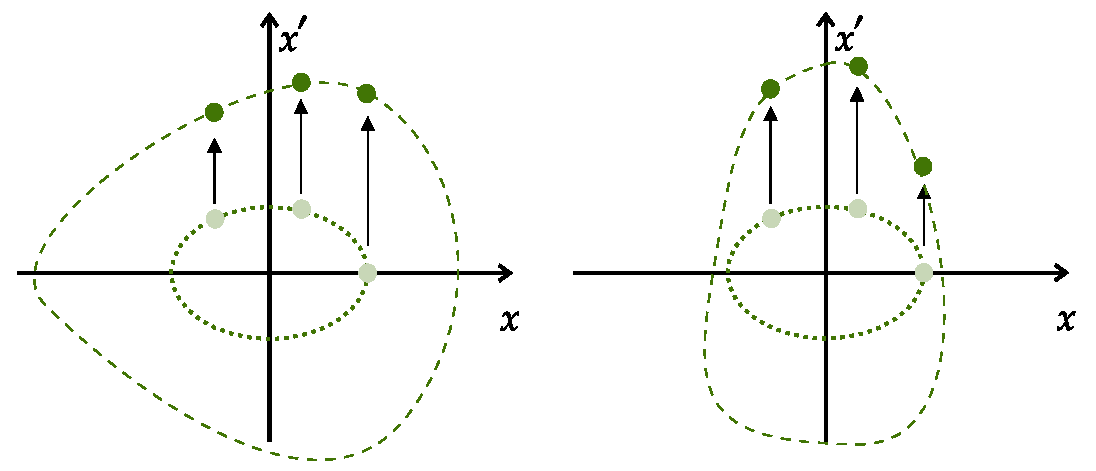
\includegraphics[width=0.9\textwidth]{Images/elastic_phase_space_distortion.pdf}
    \caption[Expected phase space ellipse distortions vs. hypothetically realized distortions.]{Expected phase space ellipse distortions, in the left. Hypothetically realized distortions, preferentially along the $x^\prime$ axis, in the right.}
    \label{fig:expected_vs_reality_DA}
\end{figure}
\section{Injection efficiency optimization}
\label{sec:injeff_opt}
The initial attempt to optimize the Dynamic Aperture (DA) by minimizing beam loss revealed that the optimization procedure did not enhance injection efficiency, suggesting there was no effect over the DA in the $x$ direction. This led to the decision to use the injection efficiency itself as the objective function.

In this setup, changes are made to the sextupoles, and each evaluation of the objective function involves the taking the average of efficiency of 5 injection pulses into the storage ring. With this configuration, the expected error of the objective function was approximately $\sigma=1\%$.

The ideia behind optimizing injection efficiency is to change the injection conditions to deliberately reduce the efficiency by delivering the incoming beam right on the DA border. The subsequent improvement in efficiency would be a result of DA enlargement. Extra attention was given to the injection conditions and the anticipated beam positions in phase space during this process, taking into account the seemingly elastic nature of the Dynamic Aperture (DA) boundary. The injection efficiency was intentionally reduced by lowering the NLK kick strength, which results in placing the beam slightly above the nominal value of $x^\prime\approx 0$. In practice, a value of $x^\prime\approx 0.100~\unit{mrad}$ was typically set in the experiments. Consequently, the beam was injected at the upper-left border of the $(x,x^\prime)$ aperture, as illustrated in Fig.~\ref{fig:inj_cond}. The efficiency under such conditions was approximately $30\%$.

The expectation was that maximizing injection efficiency in these conditions would correspond to a more even enlargement of the DA in both the $x$ and $x^{\prime}$ directions, stretching the boundary diagonally in the upper-left quadrant. This is in contrast to the previous attempt, where the enlargement seemed to occur preferentially along the $x^\prime$ direction. Once the procedure is complete, the DA is anticipated to be larger than in the initial state, and it is expected that injection under nominal conditions $(x, x^\prime)\approx(-8~\unit{mm}, 0)$ would be significantly more efficient.
\begin{figure}[tb]
    \centering
    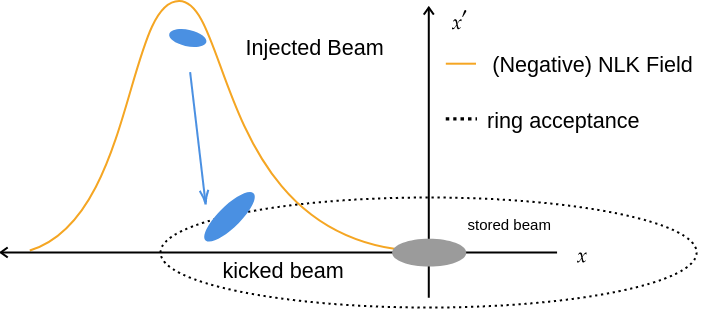
\includegraphics[width=0.7\columnwidth]{Images/inj_cond.png}
    \caption[Injection conditions for DA optimization.]{Injection conditions for DA optimization.}
    \label{fig:inj_cond}
\end{figure}

A significant difference from the early attempt was the exclusion of families SFP1 and SFB1 as knobs in the optimization experiments. This decision was made upon realizing that these families operate near their saturation strengths, where hysteresis effects become prominent, as discussed in Section~\ref{subsubsec:compensation}.

The optimization experiments were conducted in the machine with the nominal tunes $(\nu_x,\nu_y)=(49.08, 14.14)$, referred to as Working Point 1 (WP1), as well as in the tunes $(49.20, 14.25)$ and $(49.16, 14.22)$, denoted as Working Points 2 (WP2) and 3 (WP3), respectively. As mentioned earlier, the goal was to explore a different optics configuration with smaller orbit amplification factors to enhance orbit stability. Part of the results reported below have been presented in ref.~\cite{velloso_online_2023}.

\subsection{Optimization in Working Point 1 (49.08, 14.14)}
The knob selection scheme followed the 13-dimensional search space of Constraint Scheme I, as detailed in Section~\ref{subsubsec:nullspace}. Three optimization experiments were conducted, resulting in three optimized configurations. In Run 1, the optimization began with the reference sextupole configurations loaded in the machine. The machine underwent linear optics and orbit corrections before initiating each run's optimization process.

The optimization was launched and once the best injection efficiency was achieved and no indication of further improvement was at sight, the run was halted and the best-performing sextupole configuration was saved. These optimal configurations are referred to as "solutions".

The magnets were standardized, and the solution from Run 1 was implemented in the machine. Run 2 commenced with the solution from Run 1. Since the Run 1 solution improved the efficiency, the beam's horizontal offset during injection was further increased in the negative direction to reduce the efficiency by shifting the beam toward the border of the expectedly enlarged DA. The same procedure was replicated for Run 3, which initiated from the solution obtained in Run 2. Figure~\ref{fig:wp1_history} shows the history of the objective function (average efficiency of 5 injection pulses) throughout the optimization runs at Working Point 1.
\begin{figure}[tb]
    \centering
    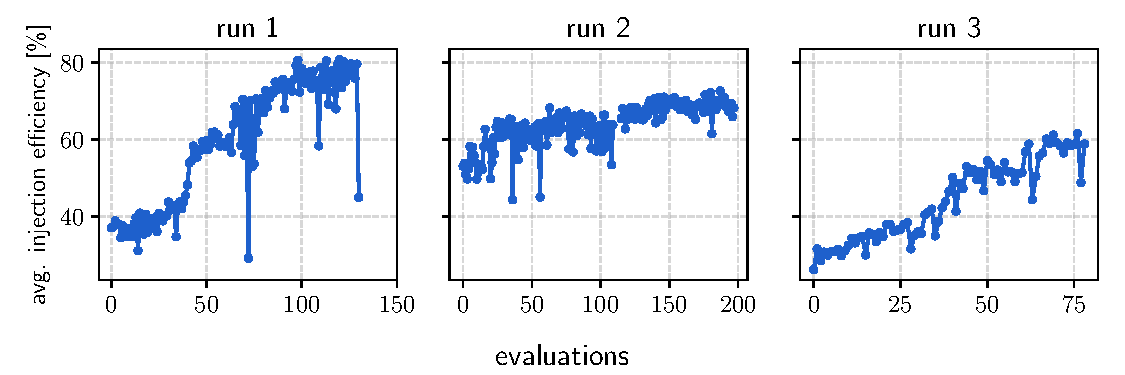
\includegraphics[width=\columnwidth]{Images/wp1_objfunc_hist.pdf}
    \caption[Objective function history during the RCDS runs in WP1.]{Objective function history during the RCDS runs in WP1.}
    \label{fig:wp1_history}
\end{figure}
\subsubsection{Characterization of solutions}
For each of the optimal configurations identified in Runs 1, 2, and 3, as well as for the non-optimized reference configuration (ref. config.), turn-by-turn (TbT) BPM data of the stored beam subjected to horizontal kicks from the dipolar kicker was collected. The DCCT current monitor allowed the determination of the current losses as a function of the horizontal kicks strengths, which is shown in Fig.~\ref{fig:loss_kicks} for the three runs. These curves characterize the beam's resilience to kicks.
\begin{figure}[tb]
    \centering
    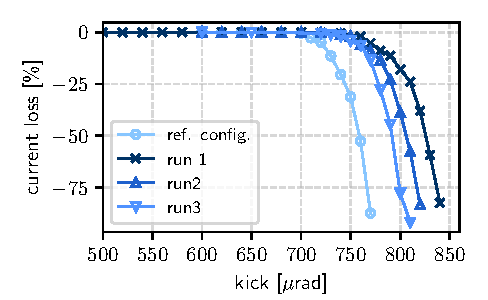
\includegraphics[width=0.6\columnwidth]{Images/WEPL087_f1.pdf}
    \caption[Current losses vs. horizontal dipole kick for the ref. config. and for the RCDS solutions at WP 1.]{Current losses vs. horizontal dipole kick for the ref. config. and for the RCDS solutions at WP 1.}
       \label{fig:loss_kicks}
\end{figure}

TbT data also allowed for the reconstruction of the $(x,x^\prime)$ phase space of the beam under the influence of the kicks. Using two BPMs at the ends of an empty ID straight section, the position and angle of the beam were determined at each turn. Figure~\ref{fig:oldtunes_phase} shows the measured phase spaces for the ref. config. and the best configurations found during run 1, 2, and 3, at the storage ring fifth straight section (SA05), which is a high-beta section with optics identical to that of the injection point. In the measurement, the beam was under the influence of kicks rendering approximately the same current loss of $12\%$.
\begin{figure}[tb]
    \centering
        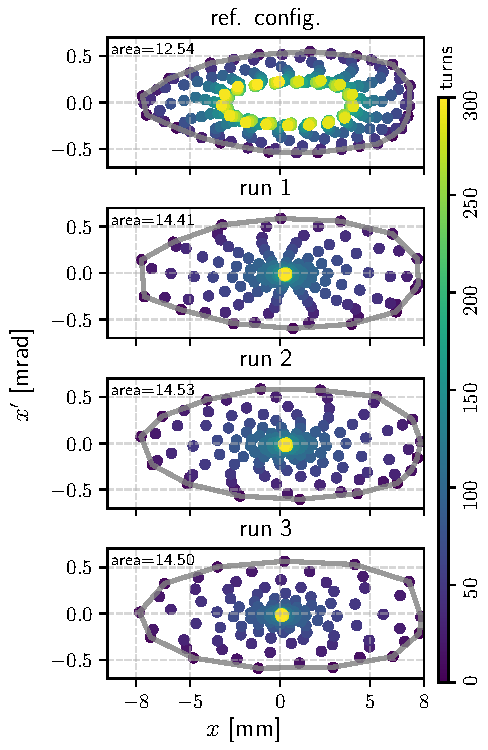
\includegraphics[width=\textwidth]{Images/WEPL087_f2.pdf}
        \caption[Measured phase space at SA05 high-beta straight section for the ref. config. and the best RCDS configurations of runs 1, 2 and 3 in WP 1.]{Measured phase space at SA05 high-beta straight section for the ref. config. and the best RCDS configurations of runs 1, 2 and 3 in WP 1. Color-map indicates the turns. The areas are in $\unit{mm}~\unit{mrad}$. The beam was being kicked horizontally at $730~\unit{\micro rad}$ in the ref. config, $790~\unit{\micro rad}$ in run 1, $780~\unit{\micro rad}$ in run 2, and $770~\unit{\micro rad}$, in run 3. Loss rates of  $12\%, 11\%, 13\%$ and $13\%$.}
        \label{fig:oldtunes_phase}
\end{figure}

Table~\ref{table1} compiles the injection efficiencies achieved for each configuration during off-axis NLK injection under normal injection conditions ($x\approx -8~\unit{mm}$, $x^\prime\approx 0 $).
Once again, we emphasize the apparent elasticity of the phase portrait ellipse deformations: the configuration with the highest kick resilience, observed in Run 1, is not necessarily the one with the largest phase space area and best injection efficiency performance. This behavior could be explained if the phase space deformations of the ellipse at the kicker location for this sextupole setting resulted in a larger $x^\prime/x$ ratio, contributing to a greater kick acceptance and poorer injection performance compared to Run 2. In summary, increased kick resilience does not necessarily translate into an increased DA.

Lifetime at $60~\unit{mA}$ was measured at $20~\unit{hr}$ for run 2 solution, the best performing in terms of injection efficiency. The measurement revealed no impact of the optimization procedure on lifetime, since lifetime for the same conditions on the reference configuration is $21~\unit{hr}$.

Despite the precautions taken to avoid changing chromaticity during the procedure by selecting the chromaticity Jacobian null space knobs, a slight build-up was observed. Chromaticity was measured as $(2.33, 2.53)$ in the reference configuration and $(2.24, 2.39)$ in the solution obtained in Run 2. This could be attributed to minor discrepancies between the machine computer model and the actual machine, as the optimization knobs were computed using the storage ring computer model Jacobian. Despite the small changes in chromaticity, the observed values still fall within acceptable ranges according to criteria related to impedance budgets.
\todo[inline]{clarify this}

In summary, for WP1:
\begin{itemize}
    \item the solution found during run 2 rendered $98\%$ injection efficiency,
    \item increase in horizontal phase space area and horizontal kick resilience were observed,
    \item no significant effect was observed on beam lifetime,
    \item small, acceptable chromaticity changes observed.
\end{itemize}
Increase in efficiency and phase space areas and kick resilience are strong indicators of a DA enlargement. The online optimization was extremely succesful on WP1.

\begin{table}[htb]
    \caption{Injection efficiencies for sextupole configurations found during online optimzation at Working Points 1, 2 and 3.}
    \centering
    \begin{tabular}{cccccc}
    \hline
    \multicolumn{2}{c}{working point 1} & \multicolumn{2}{c}{working point 2}         & \multicolumn{2}{c}{working point 3}         \\ \hline
    configuration      & IE $[\%]$      & configuration        & IE $[\%]$            & configuration        & IE $[\%]$            \\ \hline
    ref. config.       & $88\pm8$       & initial              & $51\pm1$             & initial              &                      \\
    run 1              & $91\pm1$       & run 1                & $79\pm3$             & optimized            & $93\pm3$             \\
    run 2              & $98\pm1$       & run 2                & $65\pm1    $         &                      &                      \\
    run 3              & $87\pm3$       & \multicolumn{1}{l}{} & \multicolumn{1}{l}{} & \multicolumn{1}{l}{} & \multicolumn{1}{l}{} \\ \hline
    \end{tabular}
    \label{table1}
    \end{table}

\subsection{Optimization in Working Point 2 (49.20, 14.25)}
The storage ring tunes were adjusted to $(\nu_x, \nu_y)=(49.20, 14.25)$. The initial sextupole configuration was the same as the nominal tunes reference configuration. The new working point significantly impacted on the DA, since the injection efficiency in nominal conditions with this setup was about $50\%$, at most. Without successful optimization, it would be impossible to operate in this working point.

For the optimization experiment, the objective function was the injection efficiency with the the beam delivered at the upper-left border of the $x,x^\prime$ phase space, just as in the WP1 experiment. The optimization knobs were those of the Constraints Scheme II, discussed in \ref{subsec:knobs}, totalling 17 independent knobs.

Two optimization runs were carried out: run 1 and run 2. The sextupoles were optimized in the new tunes starting with reference sextupoles. Once the best solution from run 1 was identified, it was re-loaded in the machine and, starting from it, run 2 was launched. The objective function history throughout the optimization is shown in Fig.~\ref{fig:wp_2_history}. Several drops in efficiency can be observed in a single run. This is because, in this experiment, there were "sub-runs": whenever the objective function improvement was slow, the optimzation was paused and the injection efficiency was worsened by increasing the beam's offset in the horizontal direction during injection. This was a manner to introduce more variability to see if it could help in accelrating the rate at which the objective was maximized.
\begin{figure}[htb]
    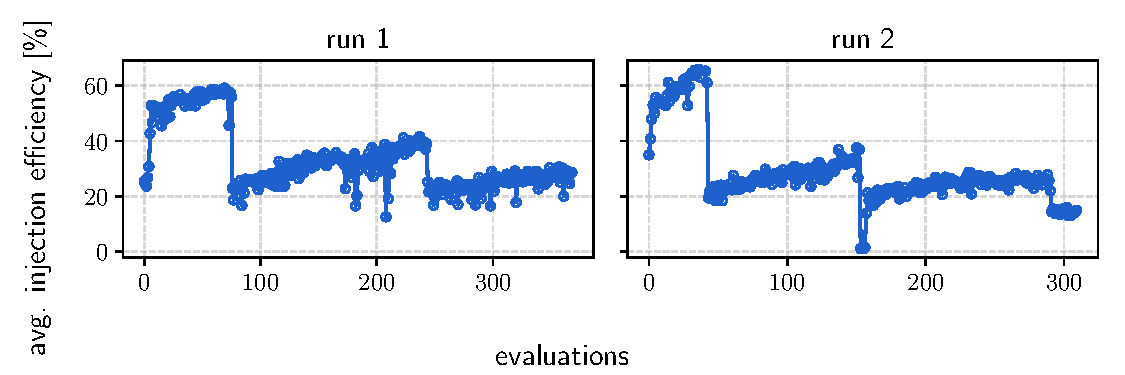
\includegraphics[width=\columnwidth]{Images/wp2_objfunc_hist.pdf}
    \caption[Objective function history during the RCDS runs in WP2.]{Objective function history during the RCDS runs in WP2.}
    \label{fig:wp_2_history}
\end{figure}
\subsubsection{Characterization of solutions}
Injection efficiency  achieved for the solutions of WP2 in nominal injection conditions is highlighted in Table~\ref{table1}. Despite the observed improvements, the best performing configuration, the solution found in run 1, still provides unsatisfactory efficiency for operation.

TbT BPM data of the kicked stored beam  in the initial configuration (non-optimized) and in each run's best solution was acquired and allowed the determination of current losses vs. kicks, shown in Fig.~\ref{fig:loss_kicks_newtunes}, and the reconstruction of phase space, shown in Fig. ~\ref{fig:newtunes_phase}. Improvements on the resilience and the phase space area can be observed in the optimized solutions.
\begin{figure}[tb]
    \centering
    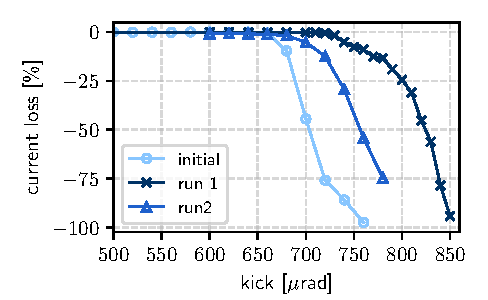
\includegraphics[width=0.6\columnwidth]{Images/WEPL087_f3.pdf}
    \caption[Current losses vs. horizontal dipole kick for the initial configuration and the RCDS solutions at WP 2.]{Current losses vs. horizontal dipole kick for the initial configuration and the RCDS solutions at WP 2.}
    \label{fig:loss_kicks_newtunes}
\end{figure}
\begin{figure}[htb]
    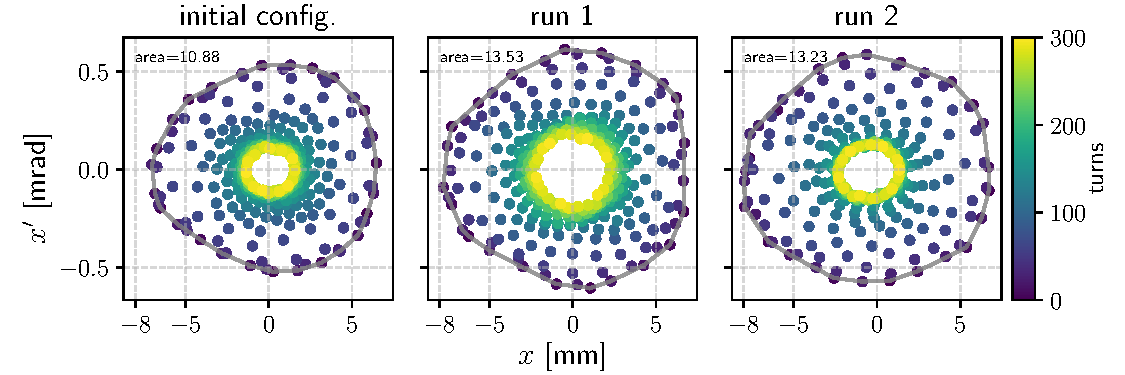
\includegraphics[width=\textwidth]{Images/WEPL087_f4.pdf}
    \caption[Measured phase space at SA05 high-beta straight section for the initial configuration and the best RCDS configurations of runs 1 and 2 in WP 2.]{Measured phase space at SA05 high-beta straight section for the initial configuration and the best RCDS configurations of runs 1 and 2 in WP 2. Color-map indicates the turns. The areas are in $\unit{mm}~\unit{mrad}$. The beam was being kicked horizontally at $680~\unit{\micro rad}$, for the initial configuration, $770~\unit{\micro rad}$ for run 1, and at $720~\unit{\micro rad}$ for run 2. Loss rates of $10\%$, $12\%$ and $12\%$, respectively}
    \label{fig:newtunes_phase}
\end{figure}

The configuration found during run 1 rendered the best injection efficiency, the largest kick resilience. It also displayed larger lifetime than the initial configuration ($21~\unit{hrs}$, run 1 vs. $18~\unit{hrs}$, initial, at $60~\unit{mA}$) which is comparable to the reference configuration lifetime at WP1. The largest phase space area increase was also observed for this solution. Still, the injection efficiency delivered by the best performing solution on this working point was quite unsatisfactory. The overall impression was that optimizing in this working point was quite difficult, as the objective function history of Fig.~\ref{fig:wp_2_history} shows. The objective rise was slow and seemd to have the $35\%$ mark as upper limit when the injection was deliberately worsened during the runs. In owther words, the DA seemed more rigid. For this reason, another working point was sought. If the idea is to increase the fraction parts of the tunes, and $(0.20, 0.25)$ seemed like overshooting towards unknown regions, optimization in the intermediate tunes between WP1 and WP2, with fractional tunes $(0.16, 0.22)$, seemed reasonable.
\subsection{Optimization in Working Point 3 (49.16, 14.22)}
From the reference configuration with corrected linear optics and orbit, the tunes were adjusted to the desired working point $(\nu_x, \nu_y)=(49.16, 13.22)$. The injection efficiency was again lower, indicating, as in WP2, deterioration of the DA when changing tunes.

The objective function was the average injection efficiency of 5 injection pulses in the same conditions as in WP1 and WP2 experiments. The optimization knobs were those of the Compensation Scheme described in section \ref{subsec:knobs}. Families SFP1 and SFB1 were not used and the search space was 13-dimensional.

Two optimization runs were carried out, starting from sextupole settings of the WP1 reference configuration. Best configuration found at run 1 was reloaded after magnets standardization and run 2 was launched. Only run 2 configuration was saved, and shall be referred to as the "optimized configuration". Figure~\ref{fig:wp3_history} shows the objective function history during the two optimization runs.
\begin{figure}[htb]
    \centering
    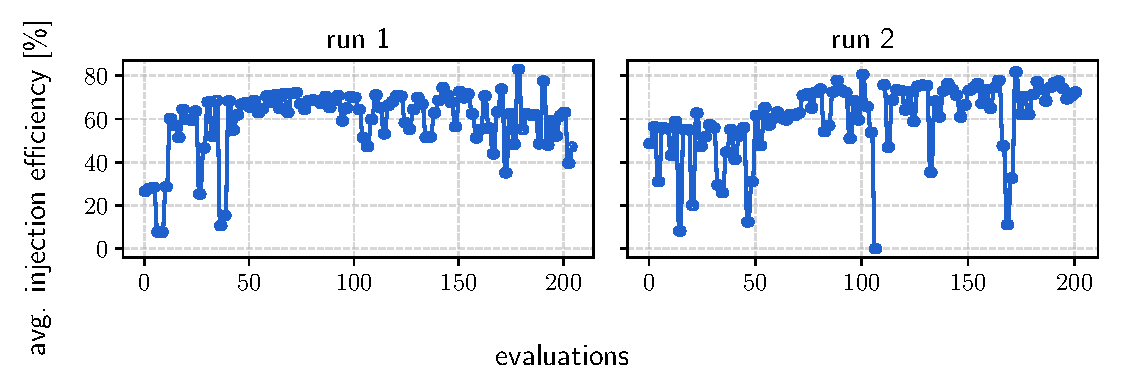
\includegraphics[width=\columnwidth]{Images/wp3_objfunc_hist.pdf}
    \caption[Objective function history during RCDS runs in WP3.]{Objective function history during RCDS runs in WP3.}
    \label{fig:wp3_history}
\end{figure}
\subsubsection{Characterization of the solution}
The optimized solution was characterized in terms of kick resilience, phase space area, injection efficiency and whether it preserved chromaticity and lifetime.  Lifetime at $60~\unit{mA}$ was measured at $19.5~\unit{hrs}$, so no significant reductions were observed. No significant chromaticity changes were observed as well. Phase space area increased, compared to the initial non-optimized configuration, and reached similar value to that of the WP1 nominal tunes reference configuration, as Fig.~\ref{fig:wp3_phase_space} shows. Kick resilience, shown in Fig.~\ref{fig:wp3_kick_res}, also improved, with a larger fraction of the beam surviving to large kicks in the range  $700-770~\unit{\mu rad}$. Finally, and most importantly, run 2 solution displayed injection efficiency of $93\pm3\%$ during nominal off-axis injection, which is acceptable for operating with this configuration.
\begin{figure}[tb]
    \centering
    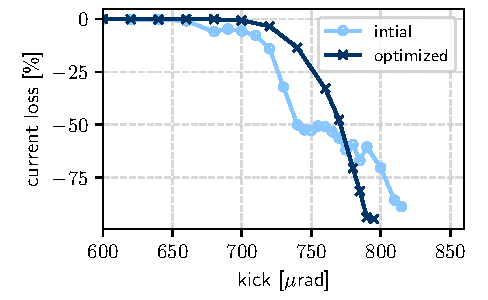
\includegraphics[width=0.6\columnwidth]{Images/wp3_kick_resilience.pdf}
    \caption[Current losses vs. horizontal dipole kick for the initial configuration and the RCDS solution at WP 3.]{Current losses vs. horizontal dipole kick for the initial configuration and the RCDS solution at WP 3.}
    \label{fig:wp3_kick_res}
\end{figure}
\begin{figure}[htb]
    \centering
    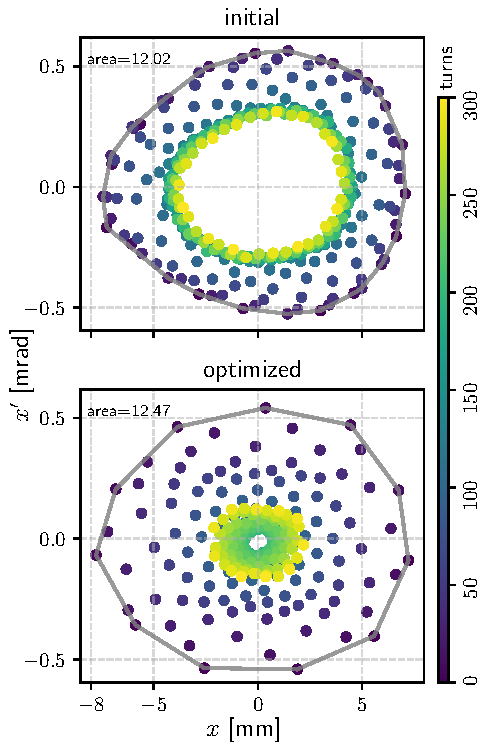
\includegraphics[width=\textwidth]{Images/wp3_phase_space.pdf}
    \caption[Measured phase space at SA05 high-beta straight section for the non-optimized configuration and the best RCDS configuration in WP 3.]{Measured phase space at SA05 high-beta straight section for the non-optimized configuration and the best RCDS configuration in WP 3. Color-map indicates the turns. The areas are in $\unit{mm}~\unit{mrad}$.}
    \label{fig:wp3_phase_space}

\end{figure}
\subsubsection{Orbit stability improvements}
The motivation for exploring higher tunes was the desirable effect of reducing orbit amplification factors to improve the overall orbit stability. Orbit stability improvements in WP3 tunes were confirmed by the orbit integrated spectrum density of the orbit data colleced with BPMs. The spectrum decreased by a factor of approximately 2, as Fig.~\ref{fig:integrated_spec}, from Ref.~\cite{liu_status_2023} shows.

Leveraging WP3, which is at the time of this writing the working point in operation at the SIRIUS storage ring, and the recent improvements of the Fast Orbit Feedback System, orbit rms variations reached the record values of less than $1\%$ of the horizontal beam size, in the horizontal plane, and less than $4\%$ of the vertical beam size in the vertical plane. Employing this WP routinely in the machine was made possible only after achieving high and reproducible injection efficiencies attending the operation demands.

\begin{figure}[htb]
    \centering
    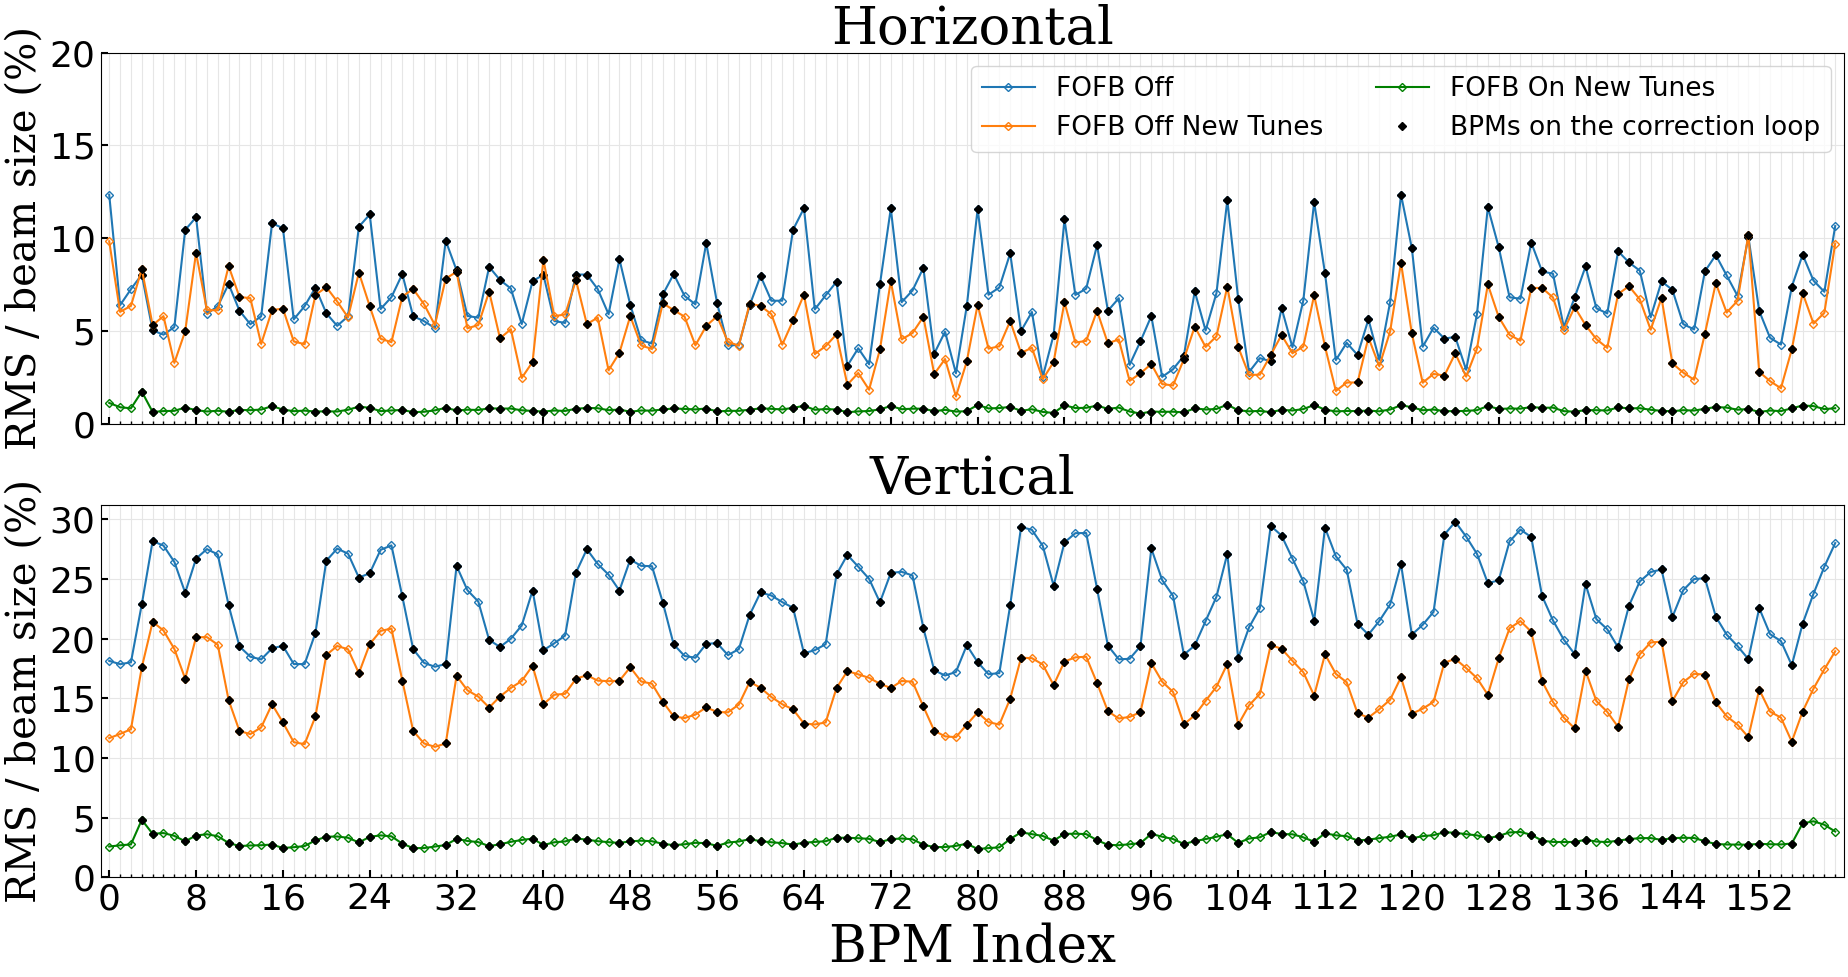
\includegraphics[width=\textwidth]{Images/WEOGA2_f5.png}
    \caption[Horizontal (vertical) RMS orbit variations in units of the horizontal (vertical) beam sizes.]{Horizontal (vertical) RMS orbit variations in units of the horizontal (vertical) beam sizes. Blue curves represents orbit variations in the nominal working point, WP1, orange curves are the orbit variations at WP3, and green curves variations at WP3 under the effects of the recentt improvements in Fast Orbit Feedback System. From Ref.~\cite{liu_status_2023}}
    \label{fig:integrated_spec}
\end{figure}

\section{Amplitude-dependent tune-shift analysis}
Online optimization is a heuristic optimization approach. The sextupole configurations found can be very different among themselves and from the nominal sextupole lattice strengths. One may wonder if any of the RCDS-optimized sextupole configurations share any common characteristic.

One intrinsic feature of nonlinear dynamics and relatively easy to experimentally access is the nonlinear tune-shifts. Specifically, the transverse amplitudes tune-shifts. By kicking the beam with the dipolar kick at high strengths and acquiring TbT BPM data one can sample the large-amplitude betatron motion and fit it in the time domain to extract the fundamental frequency, which is the tune. Repeating this analysis for  several kicks, from $500~\unit{\mu rad}$ up to $850~\unit{\mu rad}$, the amplitude-dependent tune-shift $\Delta\nu$ can be measured. Additionally, using TbT data and eq. (9) of Ref.~\cite{resende_equilibrium_2021}, the betatron action $J$ can be fitted.

This procedure was performed for each RCDS sextupole configuration in the 3 working points, specializing to the horizontal tune-shifts due to horizontal kicks. The $\Delta \nu_x$ vs. $J_x$ curves are shown by Fig.~\ref{fig:adts}. The black-curve is the expected tune-shifts for the nominal sextupole strengths. It was calculated in the storage ring computer model at each working point. The other curves were measured for each RCDS-optimized sextupole configuration with the aforementioned processing procedure.

The common feature among the curves of the best performing configurations (run 2 for WP1, run 1 for WP2 and the optimized curve for WP3) seems to be the consistent departure from the nominal model curve, towards negative tune-shifts values. This trend for tune-shifts seems to be beneficial for the actual machine.
\begin{figure}[htb]
    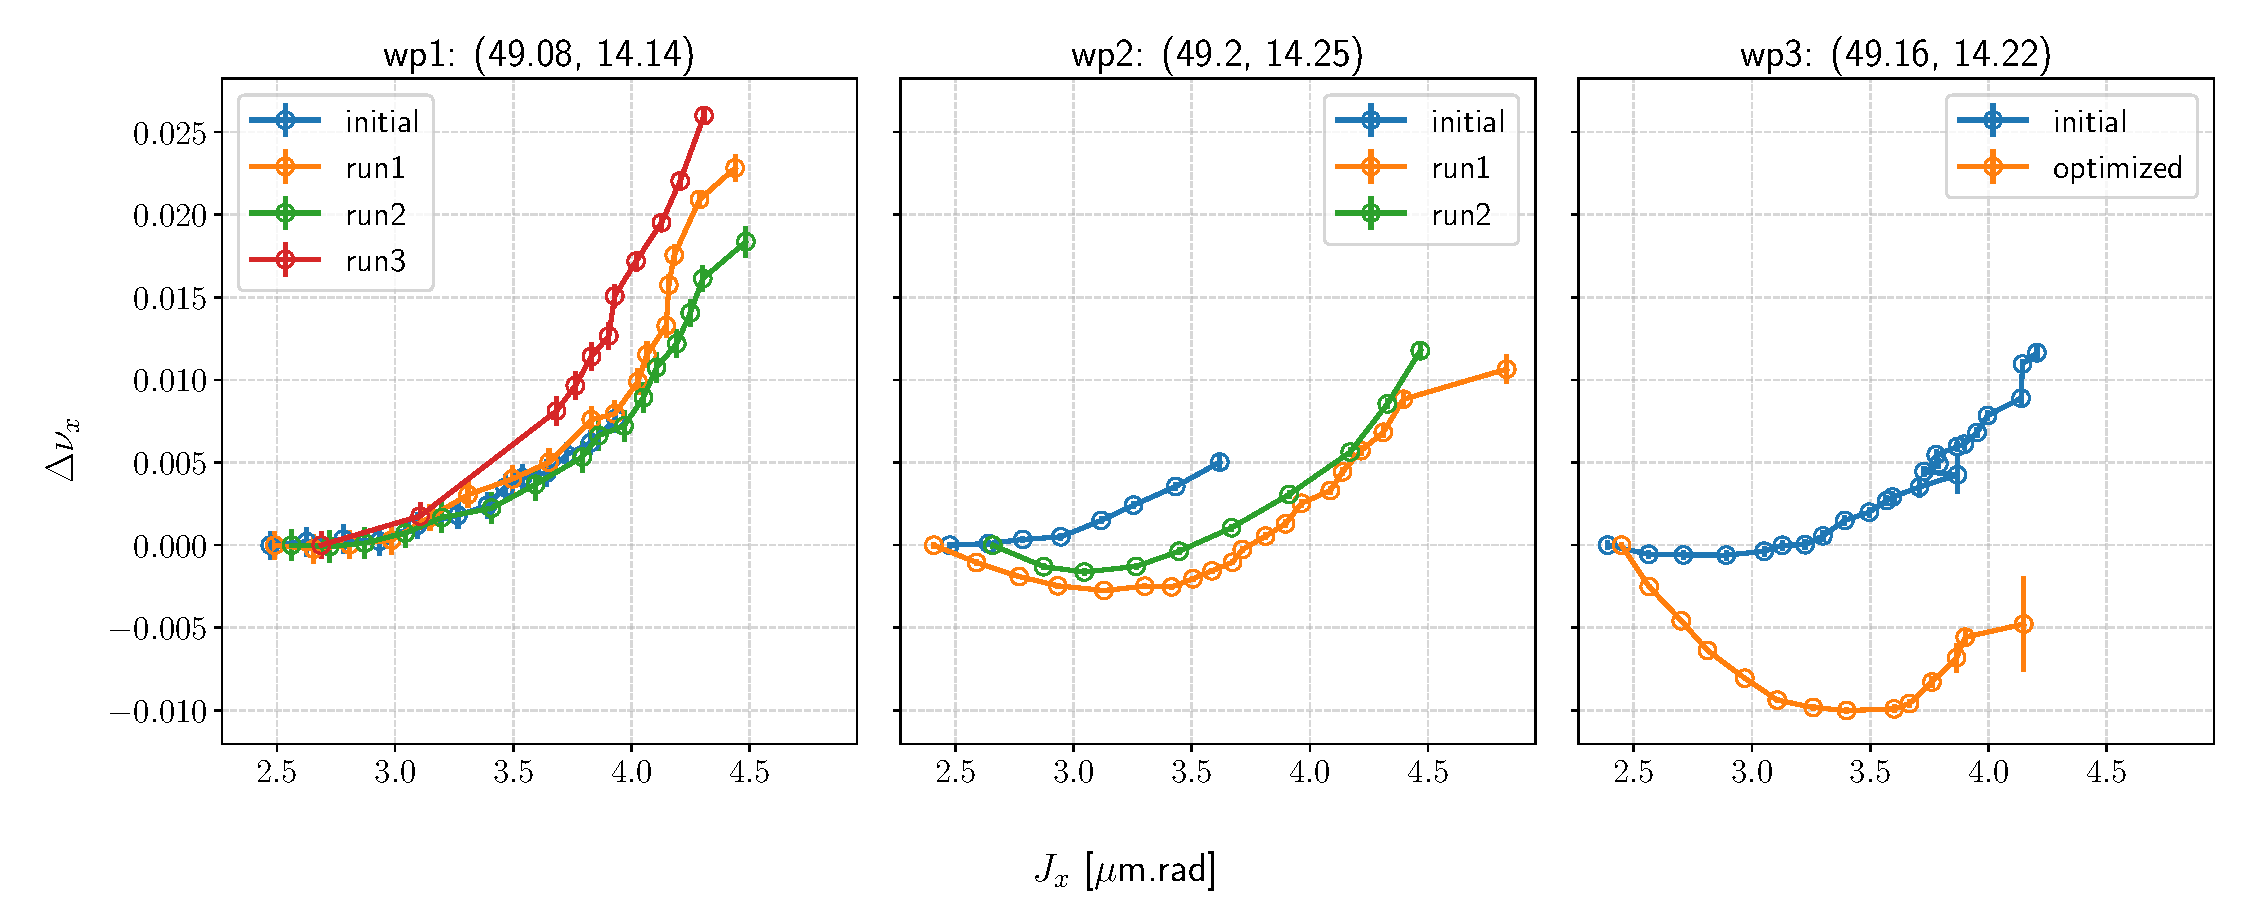
\includegraphics[width=\columnwidth]{Images/opt_configs_dtunes.pdf}
    \caption[Horizontal tune-shifts vs. horizontal betatron actions for the RCDS solutions and for the computer model in WPs 1, 2, and 3.]{Horizontal tune-shifts vs. horizontal betatron actions for the RCDS solutions and for the computer model in WPs 1, 2, and 3.}
    \label{fig:adts}
\end{figure}
